
\documentclass{article}

\title{A New Solution of Hydrogen}
\author{Brent Baccala}

\usepackage{amsmath}
\usepackage{amsfonts}

\usepackage{xcolor}
\usepackage{comment}
\usepackage{graphicx}

\usepackage[hidelinks]{hyperref}

\usepackage{tabularx}

\usepackage{longtable}

% For drawing ansatz diagrams

\usepackage{tikz}
\usetikzlibrary{calc}
\usetikzlibrary{positioning}
\usetikzlibrary{fit}
\usetikzlibrary{backgrounds}

\def\coeff{\framebox(10,10){}}
\newcommand{\tikzmark}[1]{\tikz[overlay,remember picture] \node (#1) {};}

\begin{document}
\parindent 0pt

\maketitle

\begin{abstract}
The author has developed a novel technique, based on differential algebra,
for finding exact solutions of partial
differential equations.  As an illustration of the method,
I derive a previously unknown exact solution to the simplest time-independent Schr\"odinger equation for hydrogen.
The solution, $J_0(2\sqrt{x+r})$, involves a Bessel function, is not separable, and is not in $L^2$.
\end{abstract}

\subsection*{Introduction}
\parskip 12pt

\begin{comment}
A short list of methods to find exact solutions to PDEs:

\begin{itemize}
\item separation of variables
\item method of characteristics
\item transform methods (Fourier transform on space variables)
\item symmetry methods
\item calculus of variations
\item Evans: Laplace's eq is invariant under rotations, so look for functions of r; this is a variant of sep of var
\item Evans: Poisson's eq: Green's function is constructed from radially symmetric solution to Laplace's eq
\item Evans: Poisson's eq: calculus of variations; show that solution minimizes a functional
\item Evans: heat eq: uses several scaling symmetries to justify solution form depending on a single expression
\item Evans: Duhamel's principle: separate out one variable (t) that appears like $u_t - Lu = f$ (L has no time deriv);
      form the ``retarded solution'' that represents the effect of an infinitesimal $f$, then integrate over time
\item Evans: heat eq: scaling symmetry $\rightarrow$ fundamental sol $\rightarrow$ convolution to handle arbitrary initial condition
      $\rightarrow$ Duhamel's principle to handle the inhomogenous component
\end{itemize}
\end{comment}

A short list of methods to find exact solutions to PDEs includes separation of variables,
the method of characteristics, transform methods (including Fourier transforms),
symmetry methods, Green's functions, Duhamel's principle, and the calculus of variations.
The author has developed another exact solution technique based on differential algebra
and has used it to find a new solution to one of the most well-studied equations
in mathematical physics, the Schr\"odinger equation for hydrogen.

The Schr\"odinger equation is the quantum mechanical analog of Newton's second law.
Both Newton's equation and Schr\"odinger's equation
describe the time evolution of a system
of particles interacting under the influence of forces.
Newton's classical second law $F=ma$
describes the time evolution of the position and velocity of each particle.
Schr\"odinger's quantum mechanical formulation $H\Psi=i\frac{\delta}{\delta t} \Psi$
describes the time evolution
of the wavefunction $\Psi$, which is a complex-valued function of particle position
that encodes a probability density function for
the particle positions as $|\Psi|^2$ and a probability density function
for the particle momenta as $|\hat{\Psi}|^2$.

There is no one Schr\"odinger equation any more than there is one $F=ma$.
Each physical system under consideration gives rise to a different collection
of particles and interacting forces, and a different Hamiltonian operator $H$.
Indeed, even the approximations we
make strongly determine the form of the equation for a given system.

The Hamiltonian operator $H$, so named because of its connection to Hamiltonian
mechanics, is most typically given in the form $H=T-V$, where $T$ is the
sum of the kinetic energy of all particles and $V$ is the potential energy
of the system, due to its forces.

\begin{equation*}
H=T-V
\end{equation*}

One of the simplest Schr\"odinger equations is for the hydrogen atom,
considering the electric force attraction between the nucleus and
the electronic, and ignoring all other effects.  It has the following form:

\begin{equation*}
%\label{schrodinger}
-\frac{1}{2}\nabla^2 \Psi - \frac{1}{r}\Psi = i \frac{\delta}{\delta t} \Psi
\end{equation*}

where $\Psi$ is the wavefunction, $\nabla^2$ is the Laplacian,
and $r$ is the distance between the two particles.  We use Hartree atomic units,
a system of units in which four fundamental physical constants\footnote{the reduced Planck
constant, the elementary charge, the electron mass, and the Coulumb constant} are
assigned the value of 1, in order to eliminate the need for any
conversion constants in the equation.  The unit of distance, in particular,
is {\it Bohr radii}, approximately half an Angstr\"om, a
Angstr\"om being $10^{-10}$ meters.  The first term, $-\frac{1}{2}\nabla^2 \Psi$,
is the kinetic energy operator, and the second term, $-\frac{1}{r}\Psi$, is
the potential energy term.

We can further simplify the general, time-dependent Schr\"odinger equation
by requiring that the position and momentum probability density functions
each be time-independent.  This restricts the solution to stable states
of the hydrogen atom, settles the wavefunction up to a multiple of $e^{itE}$,
where $E$ is the state's energy in Hartrees (approximately 27 eV),
and leads to the time-independent Schr\"odinger equation for hydrogen:

\begin{equation}
\label{schrodinger hydrogen}
-\frac{1}{2}\nabla^2 \Psi - \frac{1}{r}\Psi = E \Psi
\end{equation}

This equation is amenable to seperation of variables.
Using spherical coordinates and writing $\Psi$ as $\Psi=R(r)Y(\theta, \psi) = R(r)P(\theta)F(\psi)$,
substituting into \eqref{schrodinger hydrogen}, we obtain the following expansion\footnote{hyperphysics}:

\begin{equation*}
\frac{1}{R} \frac{d}{dr}\left[ r^2 \frac{dR}{dr}\right] + 2(Er^2 + r)
+ \left[\frac{1}{P\sin\theta} \frac{d}{d\theta}\left[\sin\theta\frac{dP}{d\theta}\right]+\frac{1}{F\sin^2\theta}\frac{d^2 F}{d\psi^2}\right] = 0
\end{equation*}

The first part, dependant on $r$, is the {\it radical equation}, whose solutions are, in general.
hypergeometric functions, but which, in the case of specific energy values,
simplify to polynomials in $r$
times an exponential of $r$.  It is these solutions, combined with the solution
of the second part of the equation (the colatitude equation, solved by the associated Laguerre polynomials,
and the azimuthal equation), which have been known for a hundred years, and are
hence referred to as the {\it classical solutions} to hydrogen.

\begin{figure}
\begin{center}
\begin{tabular}{ccc}
{\bf Energy}		& {\bf Wavefunction}		& {\bf Shell} \\
{\bf (Hartrees)}	& & \\
\\
$-\frac{1}{2}$		& $e^{-r}$			& 1s \\
$-\frac{1}{8}$		& $(2-r)e^{-r/2}$		& 2s \\
			& $xe^{-r/2}$			& 2p \\
			& $ye^{-r/2}$			\\
			& $ze^{-r/2}$			\\
$-\frac{1}{18}$		& $(27-18r+2r^2)e^{-r/3}$	& 3s \\
			& $(6-r)xe^{-r/3}$		& 3p \\
			& $(6-r)ye^{-r/3}$		\\
			& $(6-r)ze^{-r/3}$		\\
%%			& $(xy)e^{-r/3}$		& 3d \\
\end{tabular}
\end{center}
\end{figure}

The associated energy levels are negative because these are bound states.  Zero energy
would correspond to an electron and a proton at rest an (infinitely) large distance apart.

The classical solutions are separable, are in $L^2$, are in $C^\infty$,
and are each paired with a negative energy value, of which $-\frac{1}{2}$ is the lowest,
and corresponds to the 1s or ground state.

Yet the existance of separable solutions leaves open the existance of non-separable solutions.

It is perhaps surprising that such a well-studied equation would have fairly simple, previously
undiscovered, non-separable solutions.

I now describe the algorithm used to find the new solution of hydrogen.

\subsection*{Solution Algorithm}

Given a PDE defined by Ritt-type differential polynomials, attempt the following:

1. Select an ansatz that defines a differential space parameterized by constants (see next section)

2. Reduce the PDE modulo the differential ideal that characterizes the differential space (differential elimination step)

3. Construct a system of polynomial equations in the constants by collecting like terms in the remaining variables (projection step)

4. Construct the ideal I defined by that system of polynomial equations as generators

5. Are there any zero divisors in the differential space? (probably not)  If not, take the radical of I.

6. Construct the primary decomposition (prime decomposition if I is radical)

7. Each ideal in the primary/prime decomposition corresponds to a variety in the space of constants,
the union of which form the solution space of the PDE in the differential space.

\subsection*{The Ansatz}

Rather than attempt to derive differential equations that apply to all solutions
of the PDE, we restrict our attention to an {\bf ansatz}, which is a family of extensions
to the differential ring used to define the PDE.  These are the primary requirements
for an {\bf ansatz}:

\begin{itemize}
\item it must be formed from a finite sequence of linear ODE and algebraic extensions, and
\item it must be expressed using differential polynomials, and
\item it must be parametized only by constants
\end{itemize}

The first requirement arises because I am specifically looking for ODE based solutions,
simply because our ODE theory and practice is far beyond our PDE theory and practice.
One of the most fundamental questions to ask of a PDE, in my opinion, is can it
be solved using ODEs?  I further restrict to linear ODEs because their theory
and practice is even more refined.  Since algebraic extensions lead naturally
to nonlinear ODE extensions, if I wish to include algebraic extensions with
linear ODE, they must be included explicitly (and are).

The second requirement is natural within the context of differential algebra,
but is even more important if we wish to systematize this algorithm using
something like Rosenfeld-Gr\"obner to perform the differential reduction step.

The final requirement is meant to ensure that we can ultimately reduce this
problem to a finite-dimensional space of constants, and as we use differential
algebra throughout, we expect a system of polynomial equations in those
constants, which will be
amenable to the techniques of classical and modern algebraic geometry.

No algorithm is presently available to select an ansatz.

I've developed a graphical notation to describe an ansatz.  Blue-purple boxes
denote rings, orange boxes (whether shaded orange or not) denote ODE extensions, and green boxes denote
algebraic extensions.  A blue box drawn immediately around an orange or green box
denote the ring formed by adjoining the element defined by the orange or green box.
Polynomials are drawn as a square white box and are
connected by a line to the ring to which they belong.  A number next to
the line indicates a degree bound on the polynomial, and two numbers
separated by a slash denote a rational function.  For example, 2/2 denotes
a rational function with a second degree numerator and a second degree
denominator.

\tikzstyle{poly}=[rectangle, draw, thick, fill=white, text width=5em, align=center, rounded corners, minimum height=2em]
\tikzstyle{poly2}=[rectangle, draw, thick, fill=white, align=center, rounded corners, minimum height=2em]
\tikzstyle{ring}=[rectangle, draw=blue, thick, fill=blue!20, text width=5em,align=center, rounded corners, minimum height=2em]
\tikzstyle{element}=[rectangle, draw=orange, thick, fill=orange!20, align=center, rounded corners, minimum height=2em]
\tikzstyle{algebraic}=[rectangle, draw=green, thick, fill=green!20, align=center, rounded corners, minimum height=2em]
\tikzstyle{degree}=[]

  \begin{tikzpicture}[remember picture]
    \node (oPsi) [poly, text width=200pt] {Polynomial selected from ring: $\framebox(10,10){}\tikzmark{a}$};
    \node (ring) [ring, node distance=50pt, below of=oPsi, text width=200pt] {ring, labeled with something like\\${\mathbf C}[x,y,z]$};
    \draw[degree] (a.west) -- (a.west|-ring.north) node[right,pos=0.6] {1 (degree bound on polynomial)};

    \node (ODE extension) [element, below=of ring, text width=200pt] {ODE extension\\described by an equation and a variable};
    \node (ODE extension 2) [element, below=of ODE extension, text width=200pt] {ring generated by adjoining element\\described with an ODE};
    \node (ODE ring) [ring, fill=none, fit=(ODE extension 2)] {};
    \node (algebraic extension) [algebraic, below=of ODE extension 2, text width=200pt] {algebraic extension\\described by minimal polynomial};
    \node (algebraic extension 2) [algebraic, below=of algebraic extension, text width=200pt] {ring generated by adjoining element\\described by an algebraic extension};
    \node (algebraic ring) [ring, fill=none, fit=(algebraic extension 2), text width=200pt] {};
  \end{tikzpicture}

%%I also use a numbering system to identify the ansatzen.  This is ansatz number 5.


{\bf Ansatz 5}

Ansatz 5, used to find the new solution of hydrogen, is a second-order ODE with linear coefficients and a linear variable, i.e:

  \begin{tikzpicture}[remember picture,out=315,in=225,distance=0.4cm,node distance=40pt]
    \node (Psi) [poly, text width=100pt] {$\framebox(10,10){}\tikzmark{a}\,\Psi'' + \framebox(10,10){}\tikzmark{b}\,\Psi' + \coeff\tikzmark{c}\,\Psi$};
    \node (Qv) [ring, below of=Psi, text width=100pt] {$\mathbf{Q}[v]$};
    \node (v) [poly, right=of Qv] {$v$};
    \draw[degree] (a.west) -- (a.west|-Qv.north) node[right,pos=0.6] {1};
    \draw[degree] (b.west) -- (b.west|-Qv.north) node[right,pos=0.6] {1};
    \draw[degree] (c.west) -- (c.west|-Qv.north) node[right,pos=0.6] {1};
    \node (Psi label) [at=(v.east|-Psi.north), anchor=north east] {\Large$\Psi$};
    \begin{scope}[on background layer]
        \node (Psi block)[fit=(Psi) (Qv) (v), inner sep=10pt, element] {};
    \end{scope}
    \node (base) [ring, node distance=70pt, below=of Psi block.east, anchor=east, text width=250pt] {$\mathbf{Q}[x,y,z,r]/(r^2-x^2-y^2-z^2)$};
    \draw[degree] (v.south) -- (v.south|-base.north) node[right,pos=0.7] {1};
  \end{tikzpicture}

The structure of Ansatz 5 can be described using differential polynomials and jet notation (subscripts indicate differentiation):

\begin{equation}
\label{ansatz 5}
\begin{gathered}
\begin{comment}
\Psi_x = \frac{\Psi'}{v_x} \qquad
\Psi_y = \frac{\Psi'}{v_y} \qquad
\Psi_z = \frac{\Psi'}{v_z} \\
\Psi'_x = \frac{\Psi''}{v_x} \qquad
\Psi'_y = \frac{\Psi''}{v_y} \qquad
\Psi'_z = \frac{\Psi''}{v_z} \\
\end{comment}
\Psi_x = \Psi' v_x \qquad
\Psi_y = \Psi' v_y \qquad
\Psi_z = \Psi' v_z \\
\Psi'_x = \Psi'' v_x \qquad
\Psi'_y = \Psi'' v_y \qquad
\Psi'_z = \Psi'' v_z \\
(a_0 + a_1 v) \Psi'' + (b_0 + b_1 v) \Psi' + (c_0 + c_1 v) \Psi = 0 \\
v = v_1 x + v_2 y + v_3 z + v_4 r
\end{gathered}
\end{equation}

Essentially we introduce a new derivation with respect to $v$.
We're only interested in how $\Psi$ differentiates with this new derivation,
and that's what $\Psi'$ and $\Psi''$ tell us.  
We do not have to modify the original differential ring, except
to add $\Psi$, $\Psi'$, and $\Psi''$ as new indeterminates.
The first
two lines of equations in \eqref{ansatz 5} show how to evaluate
the derivatives of $\Psi$ and $\Psi'$ with respect to the
derivations in the differential ring (it's just the chain rule), and the third line
shows how to eliminate $\Psi''$ wherever it appears
and and replace it with an expression in $\Psi$ and $\Psi''$.
The final equation is there because $v$, too, must be degree bounded.

\subsection*{Differential Reduction Step}

I attempted to use the Rosenfeld-Gr\"obner algorithm to reduce equation \eqref{schrodinger hydrogen}
modulo \eqref{ansatz 5}, but it ultimately ran out of memory on a 96 GB computer after
30 hours.  Instead, I used Sage to construct a polynomial ring modulo the ideal
$r^2-x^2-y^2-z^2$ to handle the algebraic extension (present not in the ansatz proper,
but in the original ring used to construct the PDE).  Next I directed the software
to expand the derivatives in \eqref{schrodinger hydrogen} and substitute for $\Psi''$ and $v$
according to the ansatz.  The result is
a rational function
with a 228 term numerator and an 18 term denominator.  We ignore the denominator.  The numerator begins:

% I used a Sage-based computer program with the following ansatz.
\begin{comment}
I found this solution roughly as follows.\footnote{
I discovered an alternate form of this solution using a somewhat more complex ansatz
on January 24, 2023.  By January 26, I had established the solution in its current form.
The original ansatz produced a rational function with
a 1254 term numerator and a 36 term denominator, that gave rise to a system of 224 equations,
and was first solved using numerical approximation (scipy.optimize.root).
}

Use Cartesian coordinates.  Let $v$ be a linear polynomial in the coordinates and the root $r=\sqrt{x^2+y^2+z^2}$,
Reduce the input PDE \eqref{schrodinger} modulo differential ideal \eqref{ansatz 5}, obtaining
\end{comment}

\begin{equation}
%% -8r\Psi x^5 b_1 b_2^2 n_1 - r\Psi x^5 b_1 b_4^2 n_1 - r \Psi x^5 b_1 b_6^2 n_1 - 2r\Psi x^5 b_2 b_3 b_4 n_1 - \cdots
-2r\Psi x^3 E d_1 v_1 - 3r\Psi x^3 n_1 v_0^2 v_1 - r\Psi x^3 n_1 v_1^3 - r\Psi x^3 n_1 v_1 v_2^2 - r\Psi x^3 n_1 v_1 v_3^2 - \cdots
\end{equation}

\subsection*{Projection Step}

Having reduced our PDE \eqref{schrodinger} by the differential ideal defined by \eqref{ansatz 5},
we now wish to project our solution onto the subspace of the constants.  We're looking for
constants that will solve equation \eqref{schrodinger} for all values of $x$, $y$, $z$, $r$,
$\Psi$, and $\Psi'$, so
we collect like terms in $x$, $y$, $z$, $r$, $\Psi$, and $\Psi'$, organizing the numerator like this:

\begin{equation}
%%\left(-8 b_1 b_2^2 n_1 - b_1 b_4^2 n_1 - b_1 b_6^2 n_1 - 2 b_2 b_3 b_4 n_1 - 2b_2 b_5 b_6 n_1 \right) r\Psi x^5 - \cdots
r\Psi x^3 \left(-2 E d_1 v_1 - 3 n_1 v_0^2 v_1 - n_1 v_1^3 - n_1 v_1 v_2^2 - n_1 v_1 v_3^2\right) - \cdots
\end{equation}

The expressions in parenthesis gives us a system of equations (only one is shown)
involving the $v_i$, $d_i$, $m_i$ and $n_i$ variables that, if satisfied,
will yield a solution to \eqref{schrodinger} in the form \eqref{v ansatz} and \eqref{psi ansatz}.  Once
duplicate equations are dropped, the system has 34 equations.


%%sage: latex(matrix(eqns()).transpose())
\begin{equation}
\label{polynomial system}
\begin{array}{r}
-2 \, n_{1} v_{0}^{3} - 4 \, n_{1} v_{0} v_{1}^{2} - 4 \, n_{1} v_{0} v_{2}^{2} - 2 \, n_{1} v_{0} v_{3}^{2} - 4 \, E d_{1} v_{0} \\
-2 \, n_{1} v_{0}^{3} - 4 \, n_{1} v_{0} v_{1}^{2} - 2 \, n_{1} v_{0} v_{2}^{2} - 4 \, n_{1} v_{0} v_{3}^{2} - 4 \, E d_{1} v_{0} \\
-2 \, n_{1} v_{0}^{3} - 2 \, n_{1} v_{0} v_{1}^{2} - 4 \, n_{1} v_{0} v_{2}^{2} - 4 \, n_{1} v_{0} v_{3}^{2} - 4 \, E d_{1} v_{0} \\
-4 \, m_{1} v_{0} v_{1} v_{2} \\
-4 \, m_{1} v_{0} v_{1} v_{3} \\
-4 \, m_{1} v_{0} v_{2} v_{3} \\
-4 \, n_{1} v_{0} v_{1} v_{2} \\
-4 \, n_{1} v_{0} v_{1} v_{3} \\
-4 \, n_{1} v_{0} v_{2} v_{3} \\
-3 \, m_{1} v_{0}^{2} v_{1} -  \, m_{1} v_{1}^{3} -  \, m_{1} v_{1} v_{2}^{2} -  \, m_{1} v_{1} v_{3}^{2} \\
-3 \, m_{1} v_{0}^{2} v_{2} -  \, m_{1} v_{1}^{2} v_{2} -  \, m_{1} v_{2}^{3} -  \, m_{1} v_{2} v_{3}^{2} \\
-3 \, m_{1} v_{0}^{2} v_{3} -  \, m_{1} v_{1}^{2} v_{3} -  \, m_{1} v_{2}^{2} v_{3} -  \, m_{1} v_{3}^{3} \\
-2 \, m_{1} v_{0}^{3} - 4 \, m_{1} v_{0} v_{1}^{2} - 4 \, m_{1} v_{0} v_{2}^{2} - 2 \, m_{1} v_{0} v_{3}^{2} \\
-2 \, m_{1} v_{0}^{3} - 4 \, m_{1} v_{0} v_{1}^{2} - 2 \, m_{1} v_{0} v_{2}^{2} - 4 \, m_{1} v_{0} v_{3}^{2} \\
-3 \, n_{1} v_{0}^{2} v_{1} -  \, n_{1} v_{1}^{3} -  \, n_{1} v_{1} v_{2}^{2} -  \, n_{1} v_{1} v_{3}^{2} - 2 \, E d_{1} v_{1} \\
-3 \, n_{1} v_{0}^{2} v_{2} -  \, n_{1} v_{1}^{2} v_{2} -  \, n_{1} v_{2}^{3} -  \, n_{1} v_{2} v_{3}^{2} - 2 \, E d_{1} v_{2} \\
-3 \, n_{1} v_{0}^{2} v_{3} -  \, n_{1} v_{1}^{2} v_{3} -  \, n_{1} v_{2}^{2} v_{3} -  \, n_{1} v_{3}^{3} - 2 \, E d_{1} v_{3} \\
-2 \, m_{1} v_{0}^{3} - 2 \, m_{1} v_{0} v_{1}^{2} - 4 \, m_{1} v_{0} v_{2}^{2} - 4 \, m_{1} v_{0} v_{3}^{2} \\
- \, n_{0} v_{0}^{2} -  \, n_{0} v_{1}^{2} -  \, n_{0} v_{2}^{2} -  \, n_{0} v_{3}^{2} - 2 \, E d_{0} - 2 \, d_{1} v_{0} \\
-2 \, n_{0} v_{0} v_{1} - 2 \, d_{1} v_{1} \\
-2 \, n_{0} v_{0} v_{2} - 2 \, d_{1} v_{2} \\
-2 \, n_{0} v_{0} v_{3} - 2 \, d_{1} v_{3} \\
-2 \, d_{1} v_{0} v_{1} - 2 \, m_{0} v_{0} v_{1} \\
-2 \, d_{1} v_{0} v_{2} - 2 \, m_{0} v_{0} v_{2} \\
-2 \, d_{1} v_{0} v_{3} - 2 \, m_{0} v_{0} v_{3} \\
- \, n_{1} v_{0}^{3} - 3 \, n_{1} v_{0} v_{1}^{2} -  \, n_{1} v_{0} v_{2}^{2} -  \, n_{1} v_{0} v_{3}^{2} - 2 \, E d_{1} v_{0} \\
- \, n_{1} v_{0}^{3} -  \, n_{1} v_{0} v_{1}^{2} - 3 \, n_{1} v_{0} v_{2}^{2} -  \, n_{1} v_{0} v_{3}^{2} - 2 \, E d_{1} v_{0} \\
- \, n_{1} v_{0}^{3} -  \, n_{1} v_{0} v_{1}^{2} -  \, n_{1} v_{0} v_{2}^{2} - 3 \, n_{1} v_{0} v_{3}^{2} - 2 \, E d_{1} v_{0} \\
-2 \, d_{1} v_{0}^{2} -  \, m_{0} v_{0}^{2} -  \, m_{0} v_{1}^{2} -  \, m_{0} v_{2}^{2} -  \, m_{0} v_{3}^{2} \\
-2 \, d_{0} \\
-2 \, d_{0} v_{0} \\
- \, m_{1} v_{0}^{3} - 3 \, m_{1} v_{0} v_{1}^{2} -  \, m_{1} v_{0} v_{2}^{2} -  \, m_{1} v_{0} v_{3}^{2} \\
- \, m_{1} v_{0}^{3} -  \, m_{1} v_{0} v_{1}^{2} - 3 \, m_{1} v_{0} v_{2}^{2} -  \, m_{1} v_{0} v_{3}^{2} \\
- \, m_{1} v_{0}^{3} -  \, m_{1} v_{0} v_{1}^{2} -  \, m_{1} v_{0} v_{2}^{2} - 3 \, m_{1} v_{0} v_{3}^{2}
\end{array}
\end{equation}

\subsection*{Prime Decomposition}

\begin{comment}
I used a numerical algorithm to solve the system of equations in expectation
of it being faster for larger systems, but the system \eqref{polynomial system}
is small enough that exact methods are usable.
\end{comment}
\eqref{polynomial system} is simple enough that we can form
an ideal $I$ in $\mathbf{Q}[v_0,...,m_1,E]$ from \eqref{polynomial system}, and
Sage can calculate a Gr\"obner basis for the radical $I$ in less than a second.
While we could work with the Gr\"obner basis directly\footnote{A Gr\"obner basis
of the solution ideal in lexicographic order $E>d_i>m_i>n_i>v_i$ contains 65 polynomials.}
, I find it more
useful to study the primary decomposition, which Sage computes using
the Shimoyama-Yokoyama algorithm\footnote{Localization and Primary Decomposition of
Polynomial Ideals, {\it J. Symbolic Computation} (1996) {\bf 22}, 247–277}
as implemented in Singular.  Gr\"obner basis calculations are done
as a subalgorithm of Shimoyama-Yokoyama.

Taking the radical of the ideal simplifies both the theory and the application,
and can be justified because there are no nilpotent elements in our solution
space, which is just 11-dimensional complex space ${\mathbf C}^{11}$.  The
primary decomposition of a radical ideal is also a prime decomposition,
as the distinction between primary and prime ideals is only significant
for non-radical ideals with nilpotent elements.  Sage/Singular computes
the following decomposition into prime ideals:

\begin{verbatim}
sage: I.radical().primary_decomposition()
\end{verbatim}

\begin{subequations}
\label{ideal}
\begin{align}
& \left(n_{1}, n_{0}, m_{1}, m_{0}, d_{1}, d_{0}\right)\label{ideal:5} \\
& \left(v_{3}, v_{2}, v_{1}, v_{0}, d_{0}\right)\label{ideal:4}\\
& \left(v_{1}^{2} + v_{2}^{2} + v_{3}^{2}, v_{0}, d_{1}, d_{0}\right)\label{ideal:3}\\
& \left(v_{3}, v_{2}, v_{1}, m_{1}, m_{0} - n_{0} v_{0}, 2 d_{1} + n_{0} v_{0}, d_{0}, E n_{0} - n_{1} v_{0}\right)\label{ideal:2}\\
& \left(v_{0}^{2} - v_{1}^{2} - v_{2}^{2} - v_{3}^{2}, n_{1}, m_{1}, m_{0} - n_{0} v_{0}, d_{1} + n_{0} v_{0}, d_{0}, E\right)\label{ideal:1}
\end{align}
\end{subequations}

Several of these varieties solve the system of equations, but do not lead to a meaningful solution to the differential equation.
In brief,

\begin{itemize}
\item[\eqref{ideal:5}] sets all coefficients of the ODE to zero, so we discard it,
\item[\eqref{ideal:4}] sets the variable $v$ to zero, so we discard it,
\item[\eqref{ideal:3}] sets the coefficient of
%$\frac{d^2\Psi}{dv^2}$
$D^2\Psi$
in the ODE to zero, resulting in a first-order ODE, so we discard it, too,
\item[\eqref{ideal:2}] corresponds to the classical solutions (see below), and
\item[\eqref{ideal:1}] corresponds to our new solution (see below).

\end{itemize}

How to understand ideal \eqref{ideal:2}?  $d_0$ is an ideal generator,
so $d_0=0$, and we can always multiply our DE by a constant without affecting our result, so we can set $d_1=1$.
Likewise, we can multiply our variable $v$ by a constant and that will only change our coefficients by constants,
and $v_1=v_2=v_3=0$, so we can normalize by setting $v_0=1$.  This simplifies ideal \eqref{ideal:2} to:

\begin{equation}
\left(v_{3}, v_{2}, v_{1}, v_{0} - 1, n_{0} + 2, m_{1}, m_{0} + 2, d_{1} - 1, d_{0}, 2 E + n_{1}\right)
\end{equation}

\begin{equation}
\label{classical eq in ideal}
\begin{gathered}
v=r \\
v \Psi'' + 2 \Psi' + 2(1 + E v) \Psi = 0
\end{gathered}
\end{equation}

This is the classical radial equation obtained by seperation of variables\footnote{See
Pauling and Wilson or
\url{http://hyperphysics.phy-astr.gsu.edu/hbase/quantum/hydrad.html}}.  We use
spherical coordinates, set $\Psi = R(r)P(\theta)F(\psi)$, and obtain the above equation for $R(r)$,
though it is more commonly written in this form:

\begin{equation}
\frac{1}{R} \frac{d}{dr}\left[ r^2 \frac{dR}{dr}\right] + 2(Er^2 + r) = l(l+1)
\end{equation}

where $l$ is the orbital quantum number, which can be zero.  Set $l=0$, $v=r$ and $\Psi=R$ and
expand out the derivative to obtain \eqref{classical eq in ideal}.  Its presence here was
expected and won't be commented on further.

Ideal \eqref{ideal:1} was not expected, and contains our new solution.  Does it contain any additional solutions?
$d_0$ is an ideal generator,
so $d_0=0$, and we can set $d_1=1$, by the same logic as above.
Our coordinates are in real space, so our $v_i$ coefficients must be real (why?), so all of their squares must
be positive, and since $v_0^2-v_1^2-v_2^2-v_3^3=0$, $v_0$ must be non-zero.  So we can normalize by setting $v_0=1$.
That simplifies \eqref{ideal:1} to this ideal:

\begin{equation}
\left(v_{1}^{2} + v_{2}^{2} + v_{3}^{2} - 1, v_{0} - 1, n_{1}, n_{0} + 1, m_{1}, m_{0} + 1, d_{1} - 1, d_{0}, E\right)
\end{equation}

This ideal corresponds to the following system of equations:

\begin{equation}
\begin{gathered}
E = 0 \\
d_0 = 0 \qquad
d_1 = 1 \\
m_0 = -1 \qquad
m_1 = 0 \\
n_0 = -1 \qquad
n_1 = 0 \\
v_0 = 1 \qquad
v_1^2 + v_2^2 + v_3^2 = 1
\end{gathered}
\end{equation}

Substituting these values back into our ansatz, we conclude that $\Psi(v)$
is a solution of \eqref{schrodinger} under these conditions:

\begin{equation}
\label{related solution}
\begin{gathered}
v \frac{\delta^2\Psi}{\delta v^2} + \frac{\delta\Psi}{\delta v} + \Psi = 0 \\
v = v_1 x+ v_2 y+ v_3 z+r \\
v_1^2 + v_2^2 + v_3^2 = 1
\end{gathered}
\end{equation}

The expression $v_1 x + v_2 y + v_3 z$ is easily identified as a dot product between
the coordinate $(x,y,z)$ and the unit vector $(v_1, v_2, v_3)$ (remembering
that $v_1^2 + v_2^2 + v_3^2 = 1$).  The direction of this vector is arbitrary,
so we can orient the $x$-axis in this direction and set $(v_1, v_2, v_3) = (1,0,0)$
without loss of generality.

We now have to solve a second order ODE:

\begin{equation}
v \Psi''(v) + \Psi'(v) + \Psi(v) = 0
\end{equation}

Wolfram Mathematica\footnote{I originally used Wolfram Alpha} can now
analyze this equation and determine that it is equivalent
to the Bessel function \eqref{solution}.

\includegraphics[page=1, clip, trim=1in 9in 1in 1in, width=\textwidth]{find Bessel solution.pdf}

leading to...

\subsection*{The Main Result}
\parskip 0pt

Consider the following simple Sch\"odinger equation for the hydrogen atom:

\begin{equation}
\label{schrodinger}
-\frac{1}{2}\nabla^2 \Psi - \frac{1}{r}\Psi = E \Psi
\end{equation}

Let $J_0$ be the ordinary Bessel function $J_0$, and set

\begin{equation}
\label{solution}
\Psi = J_0(2\sqrt{x+r})
\end{equation}

where $x,y,z$ are Cartesian coordinates and $r=\sqrt{x^2+y^2+z^2}$.

\vskip 12pt

Then \eqref{solution} is an exact solution to \eqref{schrodinger}, with $E=0$.

\subsection*{Verification}

The result can be easily verified using Mathematica\footnote{A manual verification is presented in an appendix}, as follows:

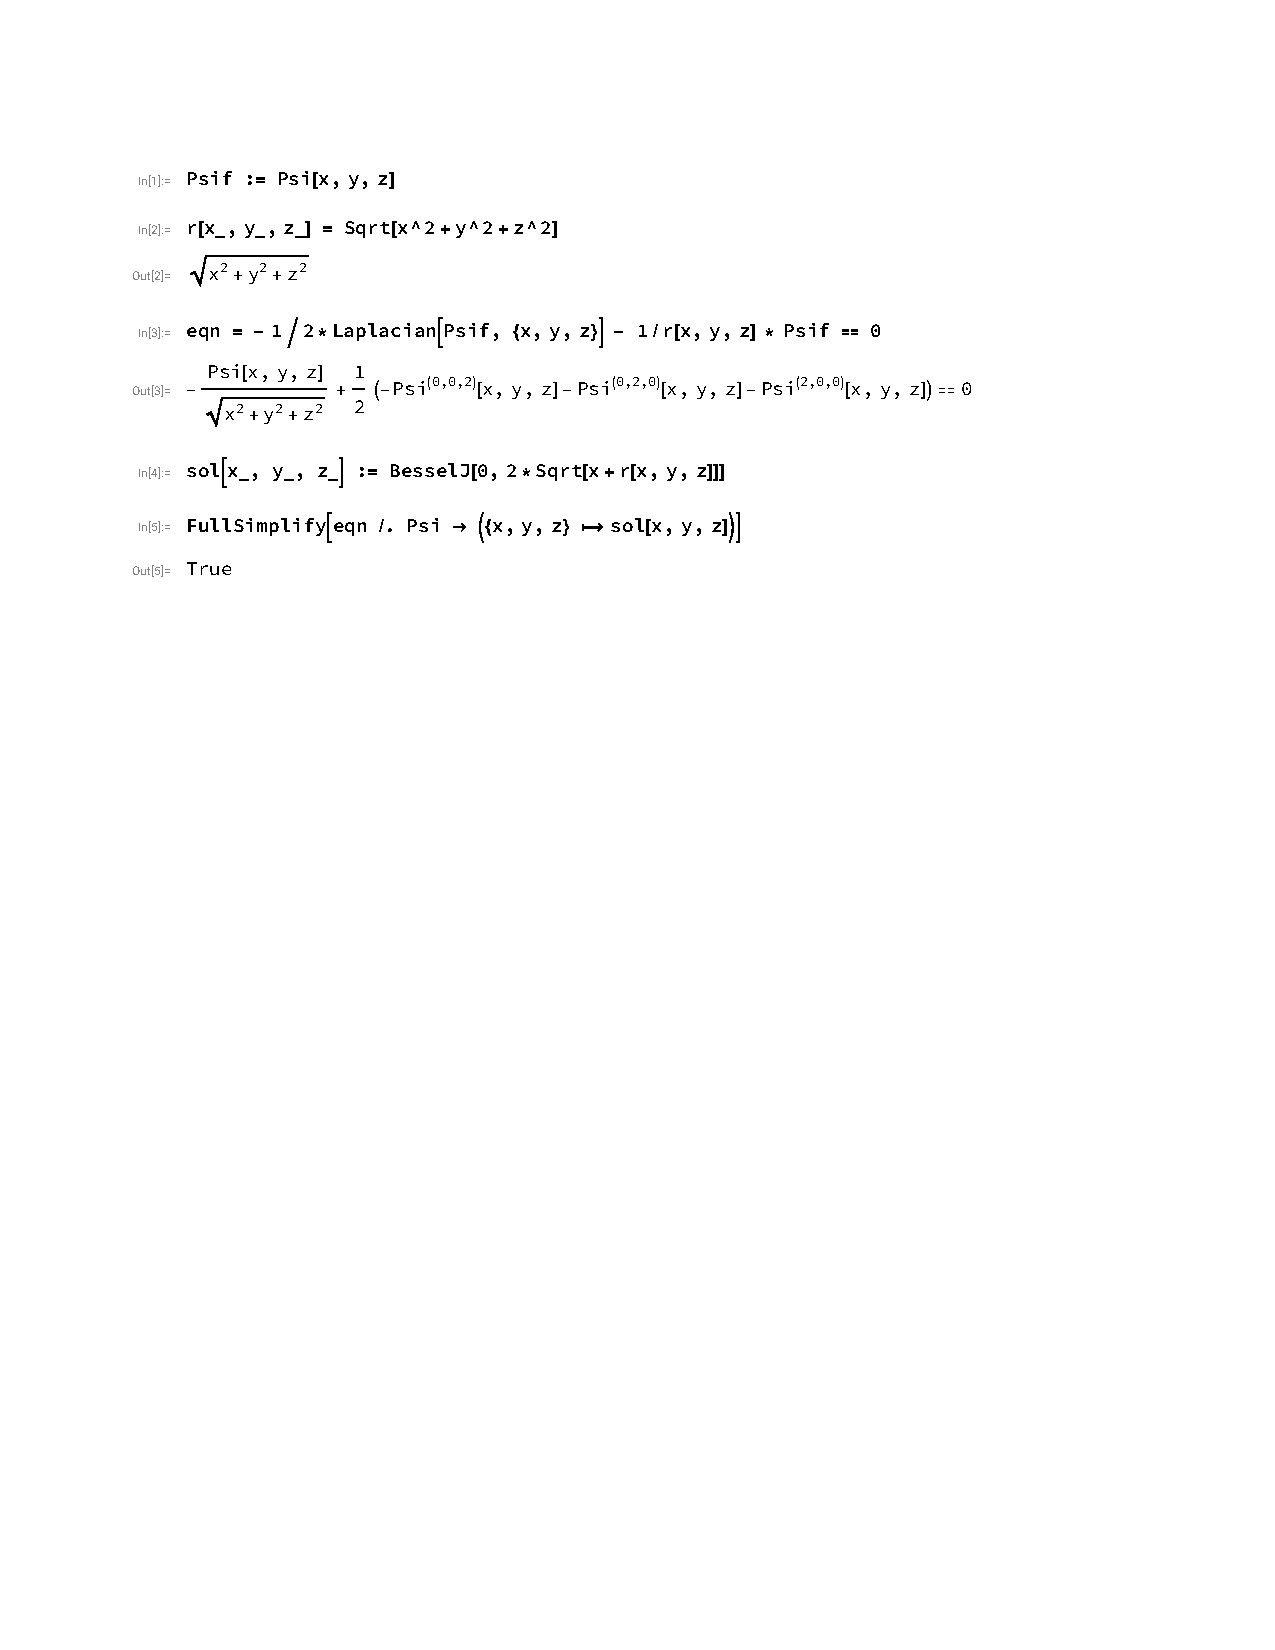
\includegraphics[page=1, clip, trim=1in 7in 1in 1in, width=\textwidth]{improved.pdf}

\subsection*{Generalization}
\parskip 12pt

The choice of $x$ is arbitrary, and any ordinary Bessel function can be used:

\begin{equation}
\label{generalized solution}
\Psi = F(2\sqrt{a_1 x+ a_2 y+ a_3 z+r})
\end{equation}

where

\begin{equation*}
a_1^2+a_2^2+a_3^2=1
\end{equation*}

and $F$ is any linear combination of the Bessel functions $J_0$ and $Y_0$.

\vskip 12pt

Any finite linear combination of functions of the form \eqref{generalized solution} also solves \eqref{schrodinger}.

\subsection*{Software}

The program used to construct the system of equations is available here:

\centerline{\url{https://github.com/BrentBaccala/helium}}

It's a Sage script that works fine with Sage 9.0 on Ubuntu 20.

%Use it to find the witness point \eqref{witness point} by
%running Sage as follows:
Use it to find ideal \eqref{ideal} by
running Sage as follows:

\begin{verbatim}
load('helium.sage')     # loads the script
prep_hydrogen(5)        # select PDE:hydrogen and ansatz:5
init()                  # finish setting everything up
I=ideal(eqns_RQQ)       # constuct ideal from equations
I.radical().primary_decomposition()
\end{verbatim}

Here are some other convenient variables and functions in the script:

\begin{verbatim}
A, B, C, V              # trial forms of various polynomials
eq_a                    # the PDE in its original form
R                       # polynomial ring over integers
F                       # fraction field of R
F_eq_a                  # the PDE modulo the ansatz
F_eq_a_n                # expanded numerator (in R)
F_eq_a_d                # expanded denominator (in R)
eqns_RQQ                # system of equations to solve
\end{verbatim}

\subsection*{Further Work}

The algorithm presented above can be used to check any PDE to see if any of its solutions
can be expressed using an ODE structured according to a specific ansatz.  This technique
is complementary to separation of variables, where we check a PDE to see if any of
its solutions can be expressed as a product of factors, each depending on only
a single variable.

As my primary interest lies in quantum mechanics, I have investigated the PDEs
that model hydrogen and helium.

For hydrogen, the PDE is $\nabla^2 \Psi - \frac{1}{r} \Psi = E \Psi$

For helium, the PDE is $\nabla_1^2 \Psi + \nabla_2^2 \Psi - \frac{2}{r_1} - \Psi \frac{2}{r_2} - \Psi \frac{1}{r_{12}} \Psi = E \Psi$,
where $\Psi=\Psi(r_1,r_2,r_{12})$ and $\nabla_i$ is the Laplacian with respect to the $i^{\rm th}$ electron.
$\Psi$ is assumed to have no angular dependence, which has been known since
at least the time of Hylleraas to be a valid assumption for the ground state.

In both cases, I use Hartree atomic units to render the equations dimensionless.

Once the PDEs have been reduced modulo the differential ideal corresponding to a selected ansatz,
the resulting system of polynomial equations must be solved.  The major techniques available are:

\begin{enumerate}
\item Exact primary decomposition

This requires the computation of Gr\"obner bases, which often fails due to memory exhaustion
(oom - out of memory) and the limitations of current

\item Numerical approximation (gradient descent / Levenberg-Marquardt)

This requires extraneous ideals/varieties to be removed as they are identified.
I'm currently exploring this approach, as it is the fastest of the three,
using the DHOST algorithm to compute Euclidean Distance polynomials for
identified varieties and use this information to drive the solutions
away from identified varieties in an attempt to find new ones.

Note that this approach, while faster than the others, will never guarantee that all solutions
to the polynomial system have been found.

\item Homotopy continuation

Bertini is a major software program, but Macaulay 2 also supports homotopy continuation.
This technique is slow but, in principle, will identify all irreducible varieties.
In practice, Bertini did not identify all five irreducible varieties for hydrogen Ansatz 5.
\end{enumerate}

\subsection*{The Ansatzen}

These are current and future ansatzen for the form of the ODE:

\begin{itemize}
\item[Ansatz 1:] Exponential of a first degree polynomial times a first degree polynomial

Expected to find 1s and 2s levels of hydrogen, $e^{-r}$ and $(2-r)e^{r/2}$

$A,B \in \mathbf{C}[x,y,z,r]; \deg A \le 1; \deg B \le 1$

$\Psi = A F; F' = F; F_x = B_x F'; F_y = B_y F'; F_z = B_z F'$

or just: $\Psi = A F; F_x = B_x F; F_y = B_y F; F_z = B_z F$

Example: $B=-r; A=1; E=-1/2$ $\qquad\Rightarrow\qquad$ $e^{-r}$

Example: $B=-r/2; A=r-2; E=-1/8$ $\qquad\Rightarrow\qquad$ $(2-r)e^{-r/2}$

\item[Ansatz 2:] Logarithm of a first degree polynomial times a first degree polynomial

$A,B \in \mathbf{C}[x,y,z,r]; \deg A \le 1; \deg B \le 1$

$\Psi = A F; F' = 1/F; F_x = B_x F'; F_y = B_y F'; F_z = B_z F'$

or just: $\Psi = A F; F_x = B_x / F; F_y = B_y / F; F_z = B_z / F$

\item[Ansatz 3,4:] Unused

\item[Ansatz 5:] Second-order ODE with linear coefficients and a linear variable

Expected to find 1s level of hydrogen, $e^{-r}$

$A,B,C,V \in \mathbf{C}[x,y,z,r]; \deg A \le 1; \deg B \le 1; \deg C \le 1; \deg V \le 1$

$\Psi = F; A F'' + B F' + C F = 0; F_x = V_x F'; F_y = V_y F'; F_z = V_z F'$

Example: $V=-r; A+C=-B; E=-1/2$ ($A, B, C \in \mathbf{C}$) $\Rightarrow$ $e^{-r}$

\item[Ansatz 6:] Second-order ODE with linear coefficients and a first-degree rational function variable

\item[Ansatz 7:] Second-order ODE with second-degree coefficients and a second-degree rational function variable

\item[Ansatz 8:] (logically before ansatz 5) First-order ODE with linear coefficients and a linear polynomial variable

\item[Ansatz 9:] (logically before ansatz 8) First-order ODE with constant coefficients and a linear polynomial variable

\item[Ansatz 10:] (logically before ansatz 7) Second-order ODE with second-degree coefficients and a second-degree polynomial variable

\item[Ansatz 11:] An second-degree algebraic extension with second-degree coefficients (involving $E$?),
followed by ansatz 7 (second-order ODE with second-degree coefficients and a second-degree rational function variable)

\item[Ansatz 12:] Two nested second-order ODEs with second-degree coefficients and a second-degree rational function variable (ansatz 7 twice)

\item[Ansatz 13:] Ansatz 11 twice

\end{itemize}

{\bf Ansatz 1}

  \begin{tikzpicture}
    \node (1base) [ring, text width=250pt] {$\mathbf{Q}[x,y,z,r]/(r^2-x^2-y^2-z^2)$};
    \node (ll-psi-a) at ($(1base.west)!0.1!(1base.east)$) {};
    \node (ll-psi) [above=of ll-psi-a.center] {.};
    \node (lr-psi) [above=of 1base.east] {.};
    \node (ur-psi) [above=of lr-psi.center] {.};
    \begin{scope}[on background layer]
        \node (Psi block)[inner sep=0pt, fit=(ll-psi.center) (ur-psi.center), element] {};
    \end{scope}
    \node (Psi) [poly2, right=of Psi block.west] {$\Psi' = \coeff\tikzmark{aa}\,\Psi$};
    \node (Psi label) [left=of Psi block.east] {\Large$\Psi$};
    \node (output) [above=of Psi.west] {\Large\fbox{$\Psi$}\tikzmark{1b}};
    \draw[degree] (Psi) -- (Psi|-1base.north) node[right,pos=0.6] {1};
    \draw[degree] (output) -- (output|-Psi block.north);
  \end{tikzpicture}

\begin{equation*}
\begin{gathered}
\Psi_x = \frac{\Psi'}{B_x} \qquad
\Psi_y = \frac{\Psi'}{B_y} \qquad
\Psi_z = \frac{\Psi'}{B_z} \\
\Psi' = \Psi \\
B = b_0 + b_1 x + b_2 y + b_3 z + b_4 r
\end{gathered}
\end{equation*}

{\bf Ansatz 9}

  \begin{tikzpicture}[remember picture,out=315,in=225,distance=0.4cm,node distance=40pt]
    \node (Psi) [poly, text width=100pt] {$\framebox(10,10){}\tikzmark{a}\,\Psi' + \coeff\tikzmark{b}\,\Psi$};
    \node (Qv) [ring, below of=Psi, text width=100pt] {$\mathbf{Q}[v]$};
    \node (v) [poly, right=of Qv] {$v$};
    \draw[degree] (a.west) -- (a.west|-Qv.north) node[right,pos=0.6] {0};
    \draw[degree] (b.west) -- (b.west|-Qv.north) node[right,pos=0.6] {0};
    \node (Psi label) [at=(v.east|-Psi.north), anchor=north east] {\Large$\Psi$};
    \begin{scope}[on background layer]
        \node (Psi block)[fit=(Psi) (Qv) (v), inner sep=10pt, element] {};
    \end{scope}
    \node (base) [ring, node distance=70pt, below=of Psi block.east, anchor=east, text width=250pt] {$\mathbf{Q}[x,y,z,r]/(r^2-x^2-y^2-z^2)$};
    \draw[degree] (v.south) -- (v.south|-base.north) node[right,pos=0.7] {1};
  \end{tikzpicture}

{\bf Ansatz 8}

  \begin{tikzpicture}[remember picture,out=315,in=225,distance=0.4cm,node distance=40pt]
    \node (Psi) [poly, text width=100pt] {$\framebox(10,10){}\tikzmark{a}\,\Psi' + \coeff\tikzmark{b}\,\Psi$};
    \node (Qv) [ring, below of=Psi, text width=100pt] {$\mathbf{Q}[v]$};
    \node (v) [poly, right=of Qv] {$v$};
    \draw[degree] (a.west) -- (a.west|-Qv.north) node[right,pos=0.6] {1};
    \draw[degree] (b.west) -- (b.west|-Qv.north) node[right,pos=0.6] {1};
    \node (Psi label) [at=(v.east|-Psi.north), anchor=north east] {\Large$\Psi$};
    \begin{scope}[on background layer]
        \node (Psi block)[fit=(Psi) (Qv) (v), inner sep=10pt, element] {};
    \end{scope}
    \node (base) [ring, node distance=70pt, below=of Psi block.east, anchor=east, text width=250pt] {$\mathbf{Q}[x,y,z,r]/(r^2-x^2-y^2-z^2)$};
    \draw[degree] (v.south) -- (v.south|-base.north) node[right,pos=0.7] {1};
  \end{tikzpicture}

{\bf Ansatz 5}

  \begin{tikzpicture}[remember picture,out=315,in=225,distance=0.4cm,node distance=40pt]
    \node (Psi) [poly, text width=100pt] {$\framebox(10,10){}\tikzmark{a}\,\Psi'' + \framebox(10,10){}\tikzmark{b}\,\Psi' + \coeff\tikzmark{c}\,\Psi$};
    \node (Qv) [ring, below of=Psi, text width=100pt] {$\mathbf{Q}[v]$};
    \node (v) [poly, right=of Qv] {$v$};
    \draw[degree] (a.west) -- (a.west|-Qv.north) node[right,pos=0.6] {1};
    \draw[degree] (b.west) -- (b.west|-Qv.north) node[right,pos=0.6] {1};
    \draw[degree] (c.west) -- (c.west|-Qv.north) node[right,pos=0.6] {1};
    \node (Psi label) [at=(v.east|-Psi.north), anchor=north east] {\Large$\Psi$};
    \begin{scope}[on background layer]
        \node (Psi block)[fit=(Psi) (Qv) (v), inner sep=10pt, element] {};
    \end{scope}
    \node (base) [ring, node distance=70pt, below=of Psi block.east, anchor=east, text width=250pt] {$\mathbf{Q}[x,y,z,r]/(r^2-x^2-y^2-z^2)$};
    \draw[degree] (v.south) -- (v.south|-base.north) node[right,pos=0.7] {1};
  \end{tikzpicture}

\begin{equation*}
\begin{gathered}
\begin{comment}
\Psi_x = \frac{\Psi'}{v_x} \qquad
\Psi_y = \frac{\Psi'}{v_y} \qquad
\Psi_z = \frac{\Psi'}{v_z} \\
\Psi'_x = \frac{\Psi''}{v_x} \qquad
\Psi'_y = \frac{\Psi''}{v_y} \qquad
\Psi'_z = \frac{\Psi''}{v_z} \\
\end{comment}
\Psi_x = \Psi' v_x \qquad
\Psi_y = \Psi' v_y \qquad
\Psi_z = \Psi' v_z \\
\Psi'_x = \Psi'' v_x \qquad
\Psi'_y = \Psi'' v_y \qquad
\Psi'_z = \Psi'' v_z \\
(a_0 + a_1 v) \Psi'' + (b_0 + b_1 v) \Psi' + (c_0 + c_1 v) \Psi = 0 \\
v = v_1 x + v_2 y + v_3 z + v_4 r
\end{gathered}
\end{equation*}

\vbox{
{\bf Ansatz 6}

  \begin{tikzpicture}[remember picture,out=315,in=225,distance=0.4cm,node distance=40pt]
    \node (Psi) [poly, text width=100pt] {$\framebox(10,10){}\tikzmark{a}\,\Psi'' + \framebox(10,10){}\tikzmark{b}\,\Psi' + \coeff\tikzmark{c}\,\Psi$};
    \node (Qv) [ring, below of=Psi, text width=100pt] {$\mathbf{Q}[v]$};
    \node (v) [poly, right=of Qv] {$v$};
    \draw[degree] (a.west) -- (a.west|-Qv.north) node[right,pos=0.6] {1};
    \draw[degree] (b.west) -- (b.west|-Qv.north) node[right,pos=0.6] {1};
    \draw[degree] (c.west) -- (c.west|-Qv.north) node[right,pos=0.6] {1};
    \node (Psi label) [at=(v.east|-Psi.north), anchor=north east] {\Large$\Psi$};
    \begin{scope}[on background layer]
        \node (Psi block)[fit=(Psi) (Qv) (v), inner sep=10pt, element] {};
    \end{scope}
    \node (base) [ring, node distance=70pt, below=of Psi block.east, anchor=east, text width=250pt] {$\mathbf{Q}[x,y,z,r]/(r^2-x^2-y^2-z^2)$};
    \draw[degree] (v.south) -- (v.south|-base.north) node[right,pos=0.7] {1/1};
  \end{tikzpicture}
}

{\bf Ansatz 7}

  \begin{tikzpicture}[remember picture,out=315,in=225,distance=0.4cm,node distance=40pt]
    \node (Psi) [poly, text width=100pt] {$\framebox(10,10){}\tikzmark{a}\,\Psi'' + \framebox(10,10){}\tikzmark{b}\,\Psi' + \coeff\tikzmark{c}\,\Psi$};
    \node (Qv) [ring, below of=Psi, text width=100pt] {$\mathbf{Q}[v]$};
    \node (v) [poly, right=of Qv] {$v$};
    \draw[degree] (a.west) -- (a.west|-Qv.north) node[right,pos=0.6] {2};
    \draw[degree] (b.west) -- (b.west|-Qv.north) node[right,pos=0.6] {2};
    \draw[degree] (c.west) -- (c.west|-Qv.north) node[right,pos=0.6] {2};
    \node (Psi label) [at=(v.east|-Psi.north), anchor=north east] {\Large$\Psi$};
    \begin{scope}[on background layer]
        \node (Psi block)[fit=(Psi) (Qv) (v), inner sep=10pt, element] {};
    \end{scope}
    \node (base) [ring, node distance=70pt, below=of Psi block.east, anchor=east, text width=250pt] {$\mathbf{Q}[x,y,z,r]/(r^2-x^2-y^2-z^2)$};
    \draw[degree] (v.south) -- (v.south|-base.north) node[right,pos=0.7] {2/2};
  \end{tikzpicture}

{\bf Ansatz 10}

  \begin{tikzpicture}[remember picture,out=315,in=225,distance=0.4cm,node distance=40pt]
    \node (Psi) [poly, text width=100pt] {$\framebox(10,10){}\tikzmark{a}\,\Psi'' + \framebox(10,10){}\tikzmark{b}\,\Psi' + \coeff\tikzmark{c}\,\Psi$};
    \node (Qv) [ring, below of=Psi, text width=100pt] {$\mathbf{Q}[v]$};
    \node (v) [poly, right=of Qv] {$v$};
    \draw[degree] (a.west) -- (a.west|-Qv.north) node[right,pos=0.6] {2};
    \draw[degree] (b.west) -- (b.west|-Qv.north) node[right,pos=0.6] {2};
    \draw[degree] (c.west) -- (c.west|-Qv.north) node[right,pos=0.6] {2};
    \node (Psi label) [at=(v.east|-Psi.north), anchor=north east] {\Large$\Psi$};
    \begin{scope}[on background layer]
        \node (Psi block)[fit=(Psi) (Qv) (v), inner sep=10pt, element] {};
    \end{scope}
    \node (base) [ring, node distance=70pt, below=of Psi block.east, anchor=east, text width=250pt] {$\mathbf{Q}[x,y,z,r]/(r^2-x^2-y^2-z^2)$};
    \draw[degree] (v.south) -- (v.south|-base.north) node[right,pos=0.7] {2};
  \end{tikzpicture}


\vbox{
{\bf Ansatz 11}

  \begin{tikzpicture}[remember picture,out=315,in=225,distance=0.4cm,node distance=40pt]
    \node (Psi) [poly, text width=100pt] {$\framebox(10,10){}\tikzmark{a}\,\Psi'' + \framebox(10,10){}\tikzmark{b}\,\Psi' + \coeff\tikzmark{c}\,\Psi$};
    \node (Qv) [ring, below of=Psi, text width=100pt] {$\mathbf{Q}[v]$};
    \node (v) [poly, right=of Qv] {$v$};
    \draw[degree] (a.west) -- (a.west|-Qv.north) node[right,pos=0.6] {1};
    \draw[degree] (b.west) -- (b.west|-Qv.north) node[right,pos=0.6] {1};
    \draw[degree] (c.west) -- (c.west|-Qv.north) node[right,pos=0.6] {1};
    \node (Psi label) [at=(v.east|-Psi.north), anchor=north east] {\Large$\Psi$};
    \begin{scope}[on background layer]
        \node (Psi block)[fit=(Psi) (Qv) (v), inner sep=10pt, element] {};
    \end{scope}
    \node (alg ext) [poly, node distance=150pt, below=of Psi.east, anchor=east, text width=100pt] {$\framebox(10,10){}\tikzmark{a}\,\gamma^2 + \framebox(10,10){}\tikzmark{b}\,\gamma + \coeff\tikzmark{c}$};
    \begin{scope}[on background layer]
        \node (alg ext element) [algebraic, fit=(alg ext) (Psi label.east|-alg ext.north), inner sep=10pt] {};
        \node (alg ext title) [node distance=20pt, above=of alg ext element.north, anchor=center, text centered, text width=250pt] {$\mathbf{Q}[x,y,z,r,\gamma]/(r^2-x^2-y^2-z^2, \framebox(10,10){}\,\gamma^2 + \framebox(10,10){}\,\gamma + \coeff\,)$};
        \node (alg ext field) [ring, fill=none, fit=(alg ext title) (alg ext element), node distance=70pt, text width=250pt] {};
    \end{scope}
    \draw[degree] (v.south) -- (v.south|-alg ext field.north) node[right,pos=0.7] {1};
    \node (base) [ring, below=of alg ext field.south east, anchor=east, text width=250pt] {$\mathbf{Q}[x,y,z,r]/(r^2-x^2-y^2-z^2)$};
    \draw[degree] (a.west) -- (a.west|-base.north) node[right,pos=0.8] {1};
    \draw[degree] (b.west) -- (b.west|-base.north) node[right,pos=0.8] {1};
    \draw[degree] (c.west) -- (c.west|-base.north) node[right,pos=0.8] {1};
  \end{tikzpicture}
}

{\bf Ansatz 12}

  \begin{tikzpicture}[remember picture,out=315,in=225,distance=0.4cm,node distance=40pt]
    \node (Psi) [poly, text width=100pt] {$\framebox(10,10){}\tikzmark{a}\,\Psi'' + \framebox(10,10){}\tikzmark{b}\,\Psi' + \coeff\tikzmark{c}\,\Psi$};
    \node (Qv) [ring, below of=Psi, text width=100pt] {$\mathbf{Q}[v]$};
    \node (v) [poly, right=of Qv] {$v$};
    \draw[degree] (a.west) -- (a.west|-Qv.north) node[right,pos=0.6] {1};
    \draw[degree] (b.west) -- (b.west|-Qv.north) node[right,pos=0.6] {1};
    \draw[degree] (c.west) -- (c.west|-Qv.north) node[right,pos=0.6] {1};
    \node (Psi label) [at=(v.east|-Psi.north), anchor=north east] {\Large$\Psi$};
    \begin{scope}[on background layer]
        \node (Psi block)[fit=(Psi) (Qv) (v), inner sep=10pt, element] {};
        %\node (Psi field) [ring, fill=none, fit=(Psi block), text width=250pt] {};
    \end{scope}

    \node (Theta) [poly, node distance=110pt, below of=Psi, text width=100pt] {$\framebox(10,10){}\tikzmark{a}\,\Theta'' + \framebox(10,10){}\tikzmark{b}\,\Theta' + \coeff\tikzmark{c}\,\Theta$};
    \node (Qu) [ring, below of=Theta, text width=100pt] {$\mathbf{Q}[u]$};
    \node (u) [poly, right=of Qu] {$u$};
    \draw[degree] (a.west) -- (a.west|-Qu.north) node[right,pos=0.6] {1};
    \draw[degree] (b.west) -- (b.west|-Qu.north) node[right,pos=0.6] {1};
    \draw[degree] (c.west) -- (c.west|-Qu.north) node[right,pos=0.6] {1};
    \node (Theta label) [at=(v.east|-Theta.north), anchor=north east] {\Large$\Theta$};
    \begin{scope}[on background layer]
        \node (Theta block)[fit=(Theta) (Qu) (u), inner sep=10pt, element] {};
        \node (Theta field) [ring, fill=none, fit=(Theta block), text width=250pt] {};
    \end{scope}

    \node (base) [ring, node distance=70pt, below=of Theta field.east, anchor=east, text width=250pt] {$\mathbf{Q}[x,y,z,r]/(r^2-x^2-y^2-z^2)$};
    \draw[degree] (v.south) -- (v.south|-Theta field.north) node[right,pos=0.7] {1};
    \draw[degree] (u.south) -- (v.south|-base.north) node[right,pos=0.7] {1};
  \end{tikzpicture}

\vbox{
   {\bf Ansatz 13}

  \begin{tikzpicture}[remember picture,out=315,in=225,distance=0.4cm,node distance=40pt]
    \node (Psi) [poly, text width=100pt] {$\framebox(10,10){}\tikzmark{a}\,\Psi'' + \framebox(10,10){}\tikzmark{b}\,\Psi' + \coeff\tikzmark{c}\,\Psi$};
    \node (alg ext) [poly, node distance=50pt, below=of Psi.east, anchor=east, text width=90pt] {$\framebox(10,10){}\tikzmark{aa}\,\gamma^2 + \framebox(10,10){}\tikzmark{bb}\,\gamma + \coeff\tikzmark{cc}$};
    \begin{scope}[on background layer]
        \node (alg ext element) [algebraic, fit=(alg ext), inner sep=5pt] {};
        \node (alg ext field) [ring, fill=none, fit=(alg ext element), node distance=70pt] {};
    \end{scope}
    \node (Qv) [ring, below of=alg ext, text width=100pt] {$\mathbf{Q}[v]$};
    \node (v) [poly, right=of Qv] {$v$};
    \draw[degree] (a.west) -- (a.west|-alg ext field.north) node[right,pos=0.6] {1};
    \draw[degree] (b.west) -- (b.west|-alg ext field.north) node[right,pos=0.6] {1};
    \draw[degree] (c.west) -- (c.west|-alg ext field.north) node[right,pos=0.6] {1};
    \draw[degree] (aa.west) -- (aa.west|-Qv.north) node[right,pos=0.8] {1};
    \draw[degree] (bb.west) -- (bb.west|-Qv.north) node[right,pos=0.8] {1};
    \draw[degree] (cc.west) -- (cc.west|-Qv.north) node[right,pos=0.8] {1};
    \node (Psi label) [at=(v.east|-Psi.north), anchor=north east] {\Large$\Psi$};
    \begin{scope}[on background layer]
        \node (Psi block)[fit=(Psi) (Qv) (v), inner sep=10pt, element, fill=none] {};
    \end{scope}
    \node (base) [ring, node distance=100pt, below=of Psi block.east, anchor=east, text width=250pt] {$\mathbf{Q}[x,y,z,r]/(r^2-x^2-y^2-z^2)$};
    \draw[degree] (v.south) -- (v.south|-base.north) node[right,pos=0.7] {1};
  \end{tikzpicture}
}

\vskip 12pt
\vbox{
   {\bf Ansatz 14}

  \begin{tikzpicture}[remember picture,out=315,in=225,distance=0.4cm,node distance=40pt]
    \node (Psi) [poly, text width=100pt] {$\framebox(10,10){}\tikzmark{a}\,\Psi'' + \framebox(10,10){}\tikzmark{b}\,\Psi' + \coeff\tikzmark{c}\,\Psi$};
    \node (ode ext) [poly, node distance=50pt, below=of Psi.east, anchor=east, text width=80pt] {$\theta' = \coeff\tikzmark{cc}$};
    \begin{scope}[on background layer]
        \node (ode ext element) [element, fit=(ode ext), inner sep=10pt] {};
        \node (ode ext field) [ring, fill=none, fit=(ode ext element), node distance=70pt] {};
    \end{scope}
    \node (Qv) [ring, node distance=50pt, below of=ode ext field, text width=100pt] {$\mathbf{Q}[v]$};
    \node (v) [poly, right=of Qv] {$v$};
    \draw[degree] (a.west) -- (a.west|-ode ext field.north) node[right,pos=0.6] {2};
    \draw[degree] (b.west) -- (b.west|-ode ext field.north) node[right,pos=0.6] {2};
    \draw[degree] (c.west) -- (c.west|-ode ext field.north) node[right,pos=0.6] {2};
    \draw[degree] (cc.west) -- (cc.west|-Qv.north) node[right,pos=0.8] {2/2};
    \node (Psi label) [at=(v.east|-Psi.north), anchor=north east] {\Large$\Psi$};
    \begin{scope}[on background layer]
        \node (Psi block)[fit=(Psi) (Qv) (v), inner sep=10pt, element, fill=none] {};
    \end{scope}
    \node (base) [ring, node distance=100pt, below=of Psi block.east, anchor=east, text width=250pt] {$\mathbf{Q}[x,y,z,r]/(r^2-x^2-y^2-z^2)$};
    \draw[degree] (v.south) -- (v.south|-base.north) node[right,pos=0.7] {2/2};
  \end{tikzpicture}
}

\vskip 12pt
\vbox{
   {\bf Ansatz 15}

  \begin{tikzpicture}[remember picture,out=315,in=225,distance=0.4cm,node distance=40pt]
    \node (Psi) [poly, text width=100pt] {$\framebox(10,10){}\tikzmark{a}\,\Psi'' + \framebox(10,10){}\tikzmark{b}\,\Psi' + \coeff\tikzmark{c}\,\Psi$};
    \node (ode ext) [poly, node distance=50pt, below=of Psi.east, anchor=east, text width=80pt] {$\framebox(10,10){}\tikzmark{aa}\,\theta'' + \framebox(10,10){}\tikzmark{bb}\,\theta' + \coeff\tikzmark{cc}\,\theta$};
    \begin{scope}[on background layer]
        \node (ode ext element) [element, fit=(ode ext), inner sep=10pt] {};
        \node (ode ext field) [ring, fill=none, fit=(ode ext element), node distance=70pt] {};
    \end{scope}
    \node (Qv) [ring, node distance=50pt, below of=ode ext, text width=100pt] {$\mathbf{Q}[v]$};
    \node (v) [poly, right=of Qv] {$v$};
    \draw[degree] (a.west) -- (a.west|-ode ext field.north) node[right,pos=0.6] {2};
    \draw[degree] (b.west) -- (b.west|-ode ext field.north) node[right,pos=0.6] {2};
    \draw[degree] (c.west) -- (c.west|-ode ext field.north) node[right,pos=0.6] {2};
    \draw[degree] (aa.west) -- (aa.west|-Qv.north) node[right,pos=0.8] {2};
    \draw[degree] (bb.west) -- (bb.west|-Qv.north) node[right,pos=0.8] {2};
    \draw[degree] (cc.west) -- (cc.west|-Qv.north) node[right,pos=0.8] {2};
    \node (Psi label) [at=(v.east|-Psi.north), anchor=north east] {\Large$\Psi$};
    \begin{scope}[on background layer]
        \node (Psi block)[fit=(Psi) (Qv) (v), inner sep=10pt, element, fill=none] {};
    \end{scope}
    \node (base) [ring, node distance=100pt, below=of Psi block.east, anchor=east, text width=250pt] {$\mathbf{Q}[x,y,z,r]/(r^2-x^2-y^2-z^2)$};
    \draw[degree] (v.south) -- (v.south|-base.north) node[right,pos=0.7] {2/2};
  \end{tikzpicture}
}

\vbox{
{\bf Ansatz 16}

  \begin{tikzpicture}[remember picture,out=315,in=225,distance=0.4cm,node distance=40pt]
    \node (Psi) [poly, text width=100pt] {$\framebox(10,10){}\tikzmark{a}\,\Psi'' + \framebox(10,10){}\tikzmark{b}\,\Psi' + \coeff\tikzmark{c}\,\Psi$};
    \node (Qv) [ring, below of=Psi, text width=100pt] {$\mathbf{Q}[v]$};
    \node (v) [poly, right=of Qv] {$v$};
    \draw[degree] (a.west) -- (a.west|-Qv.north) node[right,pos=0.6] {1};
    \draw[degree] (b.west) -- (b.west|-Qv.north) node[right,pos=0.6] {1};
    \draw[degree] (c.west) -- (c.west|-Qv.north) node[right,pos=0.6] {1};
    \node (Psi label) [at=(v.east|-Psi.north), anchor=north east] {\Large$\Psi$};
    \begin{scope}[on background layer]
        \node (Psi block)[fit=(Psi) (Qv) (v), inner sep=10pt, element] {};
    \end{scope}
    \node (alg ext) [poly, node distance=150pt, below=of Psi.east, anchor=east, text width=100pt] {$\gamma^2 = \framebox(10,10){}\tikzmark{a}$};
    \begin{scope}[on background layer]
        \node (alg ext element) [algebraic, fit=(alg ext) (Psi label.east|-alg ext.north), inner sep=10pt] {};
        \node (alg ext title) [node distance=20pt, above=of alg ext element.north, anchor=center, text centered, text width=250pt] {$\mathbf{Q}[x,y,z,r,\gamma]/(r^2-x^2-y^2-z^2, \framebox(10,10){}\,\gamma^2 + \framebox(10,10){}\,\gamma + \coeff\,)$};
        \node (alg ext field) [ring, fill=none, fit=(alg ext title) (alg ext element), node distance=70pt, text width=250pt] {};
    \end{scope}
    \draw[degree] (v.south) -- (v.south|-alg ext field.north) node[right,pos=0.7] {1};
    \node (base) [ring, below=of alg ext field.south east, anchor=east, text width=250pt] {$\mathbf{Q}[x,y,z,r]/(r^2-x^2-y^2-z^2)$};
    \draw[degree] (a.west) -- (a.west|-base.north) node[right,pos=0.8] {1};
  \end{tikzpicture}
}

\begin{comment}
%% An attempt to reform this tikz from the "bottom up" to make it easier
\vskip 12pt
\vbox{
   {\bf Ansatz 15}

  \begin{tikzpicture}

    \node (base) [ring, text width=250pt] {$\mathbf{Q}[x,y,z,r]/(r^2-x^2-y^2-z^2)$};
    \node (ll-psi-a) at ($(base.west)!0.1!(base.east)$) {};
    \node (ll-psi) [above=of ll-psi-a] {.};
    \node (Qv) [ring, right of=ll-psi] {$\mathbf{Q}[v]$};
    \node (ode ext) [poly, above=of Qv.east, anchor=east, text width=80pt] {$\framebox(10,10){}\tikzmark{aa}\,\theta'' + \framebox(10,10){}\tikzmark{bb}\,\theta' + \coeff\tikzmark{cc}\,\theta$};
  \end{tikzpicture}
}
\end{comment}

\def\R32003{$F_{32003}$}
\subsection*{Performance}
\begin{longtable}{lllll}
Ansatz 5   &Hydrogen       &Differential Elimination &Rosenfeld-Groebner    &oom, 96 GB, 30 hours\\
           &               &                         &Manual                &quick\\
           &               &Sol of constant system   &Bertini               &8.33 hours (laptop); only four components (why?)\\
           &               &                         &$\mathbb{Q}$ radical             &quick\\
           &               &                         &$\mathbb{Q}$ prime decomp        &quick\\
           &               &$\mathbb{Q}$ result                 &\multicolumn{2}{l}{5 ideals; 3 extraneous; 1 known; 1 new}\\
           &               &                         &                      &\\
           &Helium         &Differential Elimination &Manual                &30 s\\
           &               &Sol of constant system   &$\mathbb{Q}$ radical            &quick\\
           &               &$\mathbb{Q}$ result                 &\multicolumn{2}{l}{7 ideals; all extraneous}\\
           &               &                         &                      &\\
Ansatz 5.1 &Hydrogen       &Differential Elimination &Manual                &quick\\
\multicolumn{2}{l}{(2$^{\rm nd}$ degree $v$)} &Sol of constant system   &$\mathbb{Q}$ radical            &quick\\
           &               &                         &$\mathbb{Q}$ prime decomp        &quick\\
           &               &                         &                      &\\
           &Helium         &Differential Elimination &Manual                &quick\\
           &               &Sol of constant system   &$\mathbb{Q}$ radical            &quick\\
           &               &$\mathbb{Q}$ result                 &\multicolumn{2}{l}{3 ideals; not yet analyzed}\\
           &               &                         &                      &\\
Ansatz 5.2 &Hydrogen       &Differential Elimination &Manual                &quick\\
\multicolumn{2}{l}{(2$^{\rm nd}$ degree ODE)} &Sol of constant system   &$\mathbb{Q}$ radical            &quick\\
           &               &                         &$\mathbb{Q}$ prime decomp        &quick\\
           &               &                         &                      &\\
Ansatz 5.3 &Hydrogen       &Differential Elimination &Manual                &quick\\
\multicolumn{2}{l}{(both 2$^{\rm nd}$ degree)}   &Sol of constant system   &$\mathbb{Q}$ radical            &5 minutes\\
           &               &                         &$\mathbb{Q}$ prime decomp        &quick\\
           &               &                         &                      &\\
           &Helium         &Differential Elimination &Manual                &quick\\
           &               &Sol of constant system   &$\mathbb{Q}$ radical            &quick\\
           &               &$\mathbb{Q}$ result                 &\multicolumn{2}{l}{4 ideals; all extraneous}\\
           &               &                         &                      &\\
Ansatz 6   &Helium         &Differential Elimination &Manual                &10 seconds\\
           &               &Sol of constant system   &$\mathbb{Q}$ radical             &laptop crashed after $\sim$ 1 week\\
           &               &                         &Bertini               &laptop crashed after $\sim$ 1 week\\
           &               &                         &\R32003 radical        &13 min; Apr 27\\
           &               &\R32003 result            &\multicolumn{2}{l}{4 ideals; all extraneous}\\
           &               &                         &                      &\\
Ansatz 11  &Hydrogen       &Differential Elimination &Manual                &18 hours, laptop\\
           &               &Sol of constant system   &$\mathbb{Q}$ radical  &oom, 96 GB, 39 hours, c200-1\\
           &               &                         &Singular primary dec  &oom, 96 GB, c200-1\\
           &Helium         &Differential Elimination &Manual                &19 min\\
           &               &                         &                      &\\
Ansatz 12  &Hydrogen       &Differential Elimination &Manual                &quick\\
           &               &Sol of constant system   &\R32003 radical       &30 min, laptop\\
           &               &\R32003 result            &\multicolumn{2}{l}{11 ideals; not yet analyzed}\\
           &               &                         &                      &\\
Ansatz 13  &Hydrogen       &Differential Elimination &Manual                &quick\\
           &               &Sol of constant system   &$\mathbb{Q}$ radical             &quick\\
           &               &$\mathbb{Q}$ result                 &\multicolumn{2}{l}{3 ideals; all extraneous}\\
           &Helium         &Differential Elimination &Manual                &quick\\
           &               &Sol of constant system   &$\mathbb{Q}$ radical             &quick\\
           &               &$\mathbb{Q}$ result                 &\multicolumn{2}{l}{3 ideals; all extraneous}\\
           &               &                         &                      &\\
Ansatz 13.3&Hydrogen       &Differential Elimination &Manual                &quick\\
           &               &Sol of constant system   &$\mathbb{Q}$ radical             &quick\\
           &               &$\mathbb{Q}$ result                 &\multicolumn{2}{l}{3 ideals; all extraneous}\\
           &Helium         &Differential Elimination &Manual                &quick\\
           &               &Sol of constant system   &$\mathbb{Q}$ radical             &quick\\
           &               &$\mathbb{Q}$ result                 &\multicolumn{2}{l}{3 ideals; all extraneous}\\
           &               &                         &                      &\\
Ansatz 13.6&Helium         &Differential Elimination &Manual                &quick\\
           &               &Sol of constant system   &\R32003 radical             &7 min\\
           &               &$\mathbb{Q}$ result                 &\multicolumn{2}{l}{4 ideals; all extraneous}\\
           &               &                         &                      &\\
Ansatz 16  &Hydrogen       &Differential Elimination &Manual                &30 sec\\
           &               &                         &                      &\\
Ansatz 16.6&Helium         &Differential Elimination &Manual                &10 min\\
           &               &Build System of Eqns     &                      &3 hours\\
\end{longtable}

\begin{comment}
Helium 5.3: (second degree ODE coeffs and v; 6060 terms; 412 eqns; 5 min to compute radical)
   (v7, v5, v4, v3 + v6 + 2*v8, v2, v1, v0, d2, d1, d0, v6^2 + 2*v6*v8 + 2*v8^2) - leading ODE coeff zero
   (v8, v7, v5, v3 + v6, v2, d2, d1, d0, v4^2 + 4*v6^2, v1*v4 - 2*v0*v6, v0*v4 + 2*v1*v6, v0^2 + v1^2) - leading ODE coeff zero
   (v8, v7, v6, v5, v4, v3, v2, v1, v0, d0) - variable zero
   (n2, n1, n0, m2, m1, m0, d2, d1, d0) - all coeffs zero

Helium 6 R32003:

 Ideal (c3*d0 + b3*d1, c2*d0 + b2*d1, c1*d0 + b1*d1, c0*d0 + b0*d1,
        b3*c2 - b2*c3, b3*c1 - b1*c3, b2*c1 - b1*c2, b3*c0 - b0*c3, b2*c0 - b0*c2, b1*c0 - b0*c1)

given c0,c1,c2,c3, b0
  b1 = b0*c1/c0
  b2 = b0*c2/c0
  b3 = b0*c3/c0
  b-polynomial is a constant multiple (b0/c0) of c-polynomial
  b2 = b1*c2/c1
  b3 = b1*c3/c1
  b3 = b2*c3/c2
  these last three are just a further consequence of b-polynomial being a constant multiple of c-polynomial
  c0 = -b0*d1/d0
  c1 = -b1*d1/d0
  c2 = -b2*d1/d0
  c3 = -b3*d1/d0
  the constant multiple (b0/c0) also has to be (-d0/d1)

 Ideal (d1, d0, c3, b3, c1^2 + c2^2, b2*c1 - b1*c2, b1*c1 + b2*c2, b1^2 + b2^2)
   try again first order (second order coeff zero)
 Ideal (c3, c2, c1, c0)
   extraneous (denominator all zero)
 Ideal (n1, n0, m1, m0, d1, d0)
   extraneous (all ODE coeffs zero)

Helium 13.6:

[Ideal (d4, d3, d2, d1, d0, v7, v5, v4, v3 + v6 + 2*v8, v2, v1, v0, v6^2 + 2*v6*v8 + 2*v8^2)
 Ideal (d4, d3, d2, d1, d0, v8, v7, v5, v3 + v6, v2, v4^2 + 4*v6^2, v1*v4 - 2*v0*v6, v0*v4 + 2*v1*v6, v0^2 + v1^2)
 Ideal (d1, d0, v8, v7, v6, v5, v4, v3, v2, v1, v0)
 Ideal (n4, n3, n2, n1, n0, m4, m3, m2, m1, m0, d4, d3, d2, d1, d0)


Hydrogen 12 (R32003):

[Ideal (a1, a0, u0, u1^2 + u2^2 + u3^2)
 Ideal (a0, u3, u2, u1, u0)
 Ideal (n1, m1, d1 + m0, d0, v4, E, v0*n0 - m0, v0^2 - v1^2 - v2^2 - v3^2, v1^2*n0 + v2^2*n0 + v3^2*n0 - v0*m0)
 Ideal (m1, d1 - 16001*m0, d0, v4, v3, v2, v1, v0*n0 - m0, E*n0 - v0*n1, v0^2*n1 - E*m0)
 Ideal (d0, v4, v3, v2, v1, v0)
 Ideal (v4, a1, a0)
 Ideal (d1, d0, v0, u0, u3*v2 - u2*v3, v1^2 + v2^2 + v3^2, u3*v1 - u1*v3, u2*v1 - u1*v2, u1*v1 + u2*v2 + u3*v3, u1^2 + u2^2 + u3^2)
 Ideal (n1, n0, m1, m0, d1, d0)
 Ideal (d1, d0, a1, a0)
 Ideal (d1, d0, v4, v0, v1^2 + v2^2 + v3^2)
 Ideal (c1, c0, b1, b0, a1, a0)


\end{comment}

\subsection*{Draft Status}

This paper is still a draft and is being updated regularly.

\subsection*{Contact}

The author maintains a discussion page for this result on his personal blog at:

\begin{center}
\small
\url{https://www.freesoft.org/blogs/soapbox/a-new-solution-of-hydrogen/}
\end{center}

\vfill\eject
\subsection*{Appendix: Manual Verification of the Result}
For anybody wondering how Mathematica concludes that \eqref{solution} solves \eqref{schrodinger},
the claim is that $\Psi = J_0(2\sqrt{x+r}) = (J_0 \circ 2\sqrt{v}) (x+r)$ satisfies:

\begin{equation}
\label{claim}
\left(\frac{\delta^2}{\delta^2 x} + \frac{\delta^2}{\delta^2 y} + \frac{\delta^2}{\delta^2 z}\right) \Psi + \frac{2}{r}\Psi = 0
\end{equation}

\vskip 12pt

Letting $v=x+r$, we compute the first partial derivatives of $\Psi$:

\begin{equation}
\begin{gathered}
\frac{\delta \Psi}{\delta x} = \frac{d v}{d x} \frac{d}{d v} \left(J_0 \circ 2\sqrt{v}\right) = \frac{d v}{d x} J_0'(2\sqrt{v}) v^{-1/2} \\
\frac{\delta \Psi}{\delta y} = \frac{d v}{d y} \frac{d}{d v} \left(J_0 \circ 2\sqrt{v}\right) = \frac{d v}{d y} J_0'(2\sqrt{v}) v^{-1/2} \\
\frac{\delta \Psi}{\delta z} = \frac{d v}{d z} \frac{d}{d v} \left(J_0 \circ 2\sqrt{v}\right) = \frac{d v}{d z} J_0'(2\sqrt{v}) v^{-1/2}
\end{gathered}
\end{equation}

\vskip 12pt

Next we compute the partial second derivatives of $\Psi$:

\begin{equation}
\label{second partials}
\begin{gathered}
\frac{\delta^2 \Psi}{\delta x^2} = \frac{d^2 v}{d x^2} J_0'(2\sqrt{v}) v^{-1/2} + \left(\frac{d v}{d x}\right)^2 J_0''(2\sqrt{v}) v^{-1} - \frac{1}{2} \left(\frac{d v}{d x}\right)^2 J_0'(2\sqrt{v}) v^{-3/2} \\
\frac{\delta^2 \Psi}{\delta y^2} = \frac{d^2 v}{d y^2} J_0'(2\sqrt{v}) v^{-1/2} + \left(\frac{d v}{d y}\right)^2 J_0''(2\sqrt{v}) v^{-1} - \frac{1}{2} \left(\frac{d v}{d y}\right)^2 J_0'(2\sqrt{v}) v^{-3/2} \\
\frac{\delta^2 \Psi}{\delta z^2} = \frac{d^2 v}{d z^2} J_0'(2\sqrt{v}) v^{-1/2} + \left(\frac{d v}{d z}\right)^2 J_0''(2\sqrt{v}) v^{-1} - \frac{1}{2} \left(\frac{d v}{d z}\right)^2 J_0'(2\sqrt{v}) v^{-3/2}
\end{gathered}
\end{equation}

\vskip 12pt

We need to know the derivatives of $v=r+x$ with respect to the coordinates:

\vskip 12pt

\begin{equation}
\label{first v}
\begin{gathered}
\frac{d v}{d x} = \frac{d}{d x} (x+r) = 1 + \frac{x}{r} \\
\frac{d v}{d y} = \frac{d}{d y} (x+r) = \frac{y}{r} \\
\frac{d v}{d z} = \frac{d}{d z} (x+r) = \frac{z}{r}
\end{gathered}
\end{equation}

\vskip 12pt

\begin{equation}
\label{second v}
\begin{gathered}
\frac{d^2 v}{d x^2} = \frac{d}{d x} \left(1 + \frac{x}{r}\right) = \frac{r - x(x/r)}{r^2} = \frac{r^2 - x^2}{r^3} \\
\frac{d^2 v}{d y^2} = \frac{r^2 - y^2}{r^3} \\
\frac{d^2 v}{d z^2} = \frac{r^2 - z^2}{r^3}
\end{gathered}
\end{equation}

\vskip 20pt

Substituting \eqref{first v} and \eqref{second v} into \eqref{second partials}, and \eqref{second partials}
into the LHS of \eqref{claim}, we obtain:

\begin{equation*}
\begin{aligned}
&\frac{d^2 v}{d x^2} J_0'(2\sqrt{v}) v^{-1/2} + \left(\frac{d v}{d x}\right)^2 J_0''(2\sqrt{v}) v^{-1} - \frac{1}{2} \left(\frac{d v}{d x}\right)^2 J_0'(2\sqrt{v}) v^{-3/2} \\
+& \frac{d^2 v}{d y^2} J_0'(2\sqrt{v}) v^{-1/2} + \left(\frac{d v}{d y}\right)^2 J_0''(2\sqrt{v}) v^{-1} - \frac{1}{2} \left(\frac{d v}{d y}\right)^2 J_0'(2\sqrt{v}) v^{-3/2} \\
+& \frac{d^2 v}{d z^2} J_0'(2\sqrt{v}) v^{-1/2} + \left(\frac{d v}{d z}\right)^2 J_0''(2\sqrt{v}) v^{-1} - \frac{1}{2} \left(\frac{d v}{d z}\right)^2 J_0'(2\sqrt{v}) v^{-3/2} \\
+& \frac{2}{r} J_0(2\sqrt{v})
\end{aligned}
\end{equation*}

\begin{equation*}
\begin{aligned}
=&\frac{r^2-x^2}{r^3} J_0'(2\sqrt{v}) v^{-1/2} + (1+\frac{x}{r})^2 J_0''(2\sqrt{v}) v^{-1} - \frac{1}{2} (1+\frac{x}{r})^2 J_0'(2\sqrt{v}) v^{-3/2} \\
&+ \frac{r^2-y^2}{r^3} J_0'(2\sqrt{v}) v^{-1/2} + \left(\frac{y}{r}\right)^2 J_0''(2\sqrt{v}) v^{-1} - \frac{1}{2} \left(\frac{y}{r}\right)^2 J_0'(2\sqrt{v}) v^{-3/2} \\
&+ \frac{r^2-z^2}{r^3} J_0'(2\sqrt{v}) v^{-1/2} + \left(\frac{z}{r}\right)^2 J_0''(2\sqrt{v}) v^{-1} - \frac{1}{2} \left(\frac{z}{r}\right)^2 J_0'(2\sqrt{v}) v^{-3/2} \\
&+ \frac{2}{r} J_0(2\sqrt{v})
\end{aligned}
\end{equation*}

\begin{equation*}
\begin{aligned}
=&\frac{3r^2-x^2-y^2-z^2}{r^3} J_0'(2\sqrt{v}) v^{-1/2} + (1+2\frac{x}{r} +\frac{x^2}{r^2} + \frac{y^2}{r^2} + \frac{z^2}{r^2}) J_0''(2\sqrt{v}) v^{-1} \\
&- \frac{1}{2} (1+2\frac{x}{r} +\frac{x^2}{r^2}+ \frac{y^2}{r^2} + \frac{z^2}{r^2}) J_0'(2\sqrt{v}) v^{-3/2}
+ \frac{2}{r} J_0(2\sqrt{v})
\end{aligned}
\end{equation*}

\begin{equation*}
=\frac{2}{r} J_0'(2\sqrt{v}) v^{-1/2} + (2+2\frac{x}{r}) J_0''(2\sqrt{v}) v^{-1} - \frac{1}{2} (2+2\frac{x}{r}) J_0'(2\sqrt{v}) v^{-3/2} + \frac{2}{r} J_0(2\sqrt{v})
\end{equation*}

\begin{equation*}
=\frac{2}{r} J_0'(2\sqrt{v}) v^{-1/2} + 2\frac{x+r}{r} J_0''(2\sqrt{v}) v^{-1} - \frac{x+r}{r} J_0'(2\sqrt{v}) v^{-3/2}
+ \frac{2}{r} J_0(2\sqrt{v})
\end{equation*}

Remembering that $v=x+r$,

%%\begin{equation*}
%%=\frac{2}{r} J_0'(2\sqrt{v}) v^{-1/2} + 2\frac{x+r}{r} J_0''(2\sqrt{v}) v^{-1} - \frac{1}{r} J_0'(2\sqrt{v}) v^{-1/2}
%%+ \frac{2}{r} J_0(2\sqrt{v})
%%\end{equation*}

\begin{equation*}
=\frac{2}{r} J_0'(2\sqrt{v}) v^{-1/2} + \frac{2}{r} J_0''(2\sqrt{v}) - \frac{1}{r} J_0'(2\sqrt{v}) v^{-1/2}
+ \frac{2}{r} J_0(2\sqrt{v})
\end{equation*}

\begin{equation*}
=\frac{2}{r} J_0''(2\sqrt{v}) + \frac{1}{r} J_0'(2\sqrt{v}) v^{-1/2} + \frac{2}{r} J_0(2\sqrt{v})
\end{equation*}

\begin{equation*}
=\frac{2}{r} J_0''(2\sqrt{v}) + \frac{2}{r\cdot2\sqrt{v}} J_0'(2\sqrt{v}) + \frac{2}{r} J_0(2\sqrt{v})
\end{equation*}

\begin{equation}
\label{last eq in derivation}
=\frac{2}{r} \left( J_0''(2\sqrt{v}) + \frac{1}{2\sqrt{v}} J_0'(2\sqrt{v}) + J_0(2\sqrt{v})\right)
\end{equation}

Now, the ordinary Bessel function $J_0(x)$ satisfies:

\begin{equation*}
x^2 J_0''(x) + xJ_0'(x) + x^2J_0(x) = 0
\end{equation*}

dividing through by $x^2$ and changing variables, we get:

\begin{equation*}
J_0''(2\sqrt{v}) + \frac{1}{2\sqrt{v}}J_0'(2\sqrt{v}) + J_0(2\sqrt{v}) = 0
\end{equation*}

which shows that \eqref{last eq in derivation} is zero, and establishes the proof of \eqref{claim}.

\end{document}
